%% define the main template style for the document
\documentclass{article}
%% import the NIPS package for LaTeX style
\usepackage[final]{nips_2017}

%% import packages that have custom options
\usepackage[utf8]{inputenc}
\usepackage[T1]{fontenc}
\usepackage[pagebackref=true]{hyperref}
\usepackage[nolist,nohyperlinks]{acronym}
\usepackage{float}
\usepackage{graphicx}
\usepackage[caption = false]{subfig}
%% Import general packages
\usepackage{
  amsmath, amssymb, amsfonts, nicefrac,
  algorithmic, textcomp, listings, url,
  graphicx, subfig, microtype,
  booktabs, longtable
}

% Define a shortcut for inline code blocks
\def\code#1{\texttt{#1}}

%% start the document, the Markdown parser takes over from this point
\begin{document}
\title{Enhancing HiC data resolution with convolutional neural networks}

\author{
    Behnam Rasoolian \\
    Department of Software Engineering \\
    Auburn University \\
    Auburn, AL 36832 \\
    \texttt{behnam@auburn.edu} \\
    \And
    Liangliang Xu \\
    Department of Industrial Engineering \\
    Auburn University \\
    Auburn, AL 36832 \\
    \texttt{lzx0014@auburn.edu} \\
    \And
    Zheng Zhang \\
    Department of Software Engineering \\
    Auburn University \\
    Auburn, AL 36832 \\
    \texttt{zzz0069@auburn.edu} \\
}

\maketitle
\section{Abstract}
\section{Introduction}
The cell of a eukaryotic species forms a multi-granularity genome structure
in order to compactly store a very long genomic 
DNA sequence in its small nucleus. 
A \textbf{nucelotide} is the building block of
DNA. There are 4 types of nucleotides: 
C, G, A and T. 
Each pair of nucleotides in the DNA are called a \textbf{base}.
A kilo-base is a group of 1000 bases.
thousands of bases join together to form \textbf{gene loci}.
A number of loci then fold into a large
independent physical structure called \textbf{chromosome}
        (\cite{wang2013properties}).

Study of spatial conformation of chromosomes is
of high importance in the field of (computational)
biology. Although all cell is a living being
have the same sequence of genes, it is the 
3D positioning of these genes in space that
determines how the cell functions.
Roughly said,
if two genes are close to each other in
space, they can interact with each other
in order to create a certain protein that
regulates a certain task.
Thus, being
able study this 3D configuration can help
unravel mysteries of cell functioning.
However, this spatial organization of chromosomes
can not be observed through traditional 
microscopy. As an alternative,
high-throughput chromosome conformation capture
(Hi-C) has emerged as
a powerful method for studying the
3D organization of chromosomes in space.
The HiC method, which was developed by 
\cite{lieberman2009comprehensive}, 
captures interactions between
chromosomal fragments.
In this method, a chromosome is divided into
very small equally sized
sections called \textit{loci}
which is composed of 1K to 1M bases.
this method then
measures all pair-wise interaction frequencies 
across all chromosomes. 
In the past years, Hi-C method has lead to some
exiting discoveries about the topology of 
chromosomes such as presence of \textit{chromatin
loops}.
Hi-C data are usually provided as a $N \times N$
heatmap or \textit{contact matrix} where $N$ is 
the number of loci in the genome. Each cell in 
the heatmap indicates the number of \textit{interactions}
found between a pair of loci corresponding to the
rows and columns. `Resolution' of a Hi-C data
is the size of the loci the genome is
divided into.
As mentioned above
resolution can range from 1 kb to 1 Mb.
\textit{sequencing depth} is the most
important factor that determines the resolution
of data. A higher sequencing depth results in
capturing interactions between smaller loci,
thus improving the resolution of the data.
the sequencing process is costly and 
linear increase of resolution requires
quadratic increase of sequencing reads.
thus, most of the Hi-C data available have
low resolutions.

Therefore, it is required that a computational
method be developed to improve the resolution of
currently availabe Hi-C data and generate Hi-C
contact matrices of higher contrast.
Recently, deep learning 
especially Convolutional Neural Network
has emerged as a successful
method in several applications such as 
computational epigenomics. It has been
successfully used to predict DNA methylation
or gene expression patterns.

\section{The Model}
In this project, we are building upon
HiCPlus, a model proposed in 
\cite{zhang2018enhancing}, which
uses CNNs
to predict a high resolution contact
matrix from a down-sampled matrix.

In this project, however,
we used HiCPlus
model to enhance the contrast of our
low resolution data by training on
a high resolution data.

Our final purpose is to be able to
compare the three leukemic
cells with a normal cell
in terms of spatial
structure and find whether there is 
any difference in their 3D conformation
or not.
In our research, we have 5 Hi-C data sets,
belonging to
4 cell lines. Two data sets are  sequenced
from a normal cell line, one 
with high resolution (GM12878) and the
other with low resolution (GM06990)
The other three data sets are
sequenced from the same
cell lines with with three different
type of leukemia.

As mentioned above, four of the data 
sets we have are sequenced
with low depth, resulting in relatively
low resolution. 
We also have access to a high-resolution
data with much higher resolution which
is sequenced from exactly the same cell
as the normal low-resolution data that
we have. 
Therefore, we used the
HiCPlus model in \cite{zhang2018enhancing}
to enhace the contrast of our data.
We trained  the model
by using the low- and high-resolution data
of normal cells and then applied it to the 
other three cells in order to improve
their contrast.
A summary of the data and how
they are used can be 
found in table \ref{tab:data}.

\subsection{Overview of HiCPlus framework}
The inputs to the model are a low-resolution
and a high-resolution date from the same
cell line. In our project we used GM06990
for low-rosolution and GM12878 for
high-resolution data. The two data are
sequenced from the same cell lines with
the difference that the former data
cavers 979.4M bases while the latter
covers 85.1G bases, that is, the resolution
of GM12878 data is roughly 87 times higher
than the GM06990 data.
As to malignant cells,
we re-used Leukemic Hi-C libraries 
created in \cite{wang2013properties}
These libraries were sequenced 
for cases of primary human B-acute
lymphoblastic leukemia (B-ALL or ALL), 
the MHH-CALL-4 B-ALL cell
line (CALL4), 
and the follicular lymphoma cell-line (RL).
Just as \cite{wang2013properties}, 
we used normal B-cell line (GM068990)
from \cite{lieberman2009comprehensive} 
for our comparisons.
\begin{table}[]
    \centering
    \begin{tabular}{llcl}
        Data                           & Short & Resolution & Used …                     \\ \hline\hline\\
        Normal B-cell(GM12878)         & RAO   & high       & As response in training    \\[5pt]\\
        Normal B-cell(GM06990)         & MIT   & low        & As feature in training     \\[5pt]\\
        B-acute lymphoblastic leukemia & ALL   & low        & To predict high resolution \\[5pt]\\
        Follicular lymphoma cell-line  & RL    & low        & To predict high resolution \\[5pt]\\
        MHH-CALL-4                     & CALL4 & low        & To predict high resolution \\[10pt]
    \end{tabular}
    \caption{Data description}
    \label{tab:data}
\end{table}
We then fit the ConvNet model using values at 
each position in the high-resolution matrix as 
the response variable and using its 
neighbouring points from the 
low-resolution matrix as the predictors.
The authors of \cite{zhang2018enhancing}
propose a neighborhood of size $40 \times 40$
as the neighborhoold that yields best results.
Thus in order the prepare the data, we first
divided both low- and high-resolution contact
matrices into patches of size $40 \times 40$.
The model consists of 3 convolutional layers.
The design of the model is described in table
\ref{tab:modelDesign} and illustrated in 
figure \ref{fig:modelDesign}.
\begin{table}[]
    \centering
    \begin{tabular}{clcccl}
        Number   & Name           & Filter size & Filter Numbers & Strides & Output Shape \\[5pt] \hline \hline\\
        0        & input          &   -         &-               &    -    & $1\times40\times40$    \\[5pt]
        1        & conv2d1        & 9           & 8              & 1       & $8\times32\times32$    \\[5pt]
        2        & conv2d2        & 1           & 8              & 1       & $8\times32\times32$    \\[5pt]
        3        & conv2d3        & 5           & 1              & 1       & $1\times28\times28$    \\[5pt]
        4        & output\_layer  &     -       &   -            &   -     & $1\times784$     \\[30pt]
    \end{tabular}
    \caption{Desciption the CNN layers used in
    our project. The model is composed of three
    convolutional layers. The input is of shape
    $1\times40\times40$ and the output has a
    shape of $1\times784$. There are not deeply
    connected layers in the model.}
    \label{tab:modelDesign}
\end{table}
\begin{figure}[H]
    \centering
    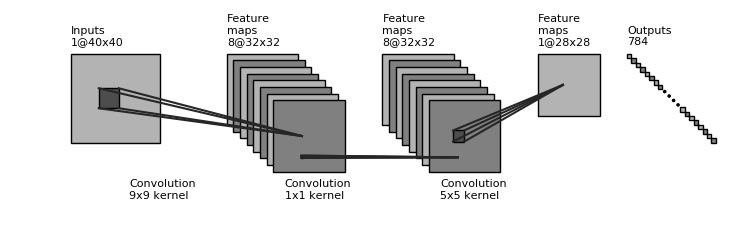
\includegraphics[width=\textwidth]{model.jpg}
    \caption{Illustration of the CNN layers used in
    our project. The model is composed of three
    convolutional layers. The input is of shape
    $1\times40\times40$ and the output has a
    shape of $1\times784$. There are not deeply
    connected layers in the model.}
    \label{fig:modelDesign}
\end{figure}
\subsection{Loss Function}
We used mean square of
differences as the loss function. As can be
seen in table \ref{tab:modelDesign} and 
\ref{fig:modelDesign}, the output of
the model hase a shape of $1 \times 784$.
In order to calculate loss function,
the model picks the middle 28 rows and columns of the
corresponding high-resolution patch and flattens
it. It then calculates the mean square of differeneces
between the output of the model and the high-resolution
sub-patch. The loss function is formulated as follows:
\begin{equation}
    \mathbb{L} = 
    \frac{1}{784}\sum_{i=1}^{784}({\hat{y}_i - y_i})^2
\end{equation}
where $\hat{y}$ denotes the output of the model and
$y$ denotes the actual high-resolution sub-patch.

We used simple gradient descent optimizer with learning
rate of \texttt{1e-5} to train the model. The choise of
optimizer did not make a great difference in the results.
Our results from using Adam optimizier also were the same
as SGD.

\section{Results}

\begin{figure}
        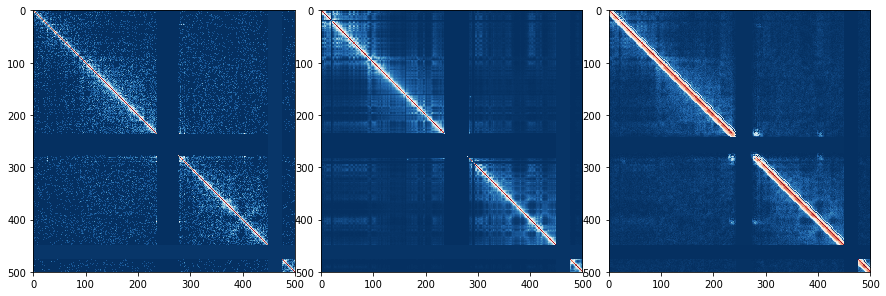
\includegraphics[width= 6in]{mit.png}
        \caption{Results of training the data on
        Normal cells. There is a total of almost
        6000 loci in a contact matrix. For the
        sake of demonstration, we only show the
        firt 500 loci. The left contact matrix is the 
        original low-resolution data. The middle one 
        is the high resolution data. and the rightmost
        picture is the result of training the model.}
        \label{fig:train}
\end{figure}
\begin{figure}
        \subfloat[]{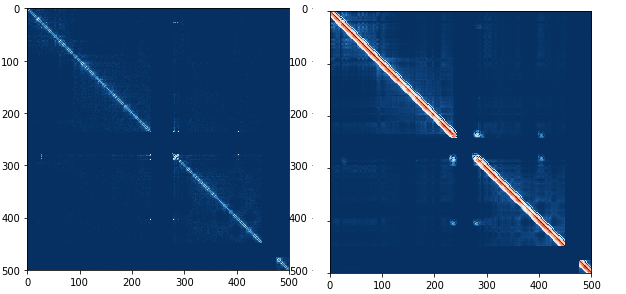
\includegraphics[width= 4in]{all.png}}\\
        \subfloat[]{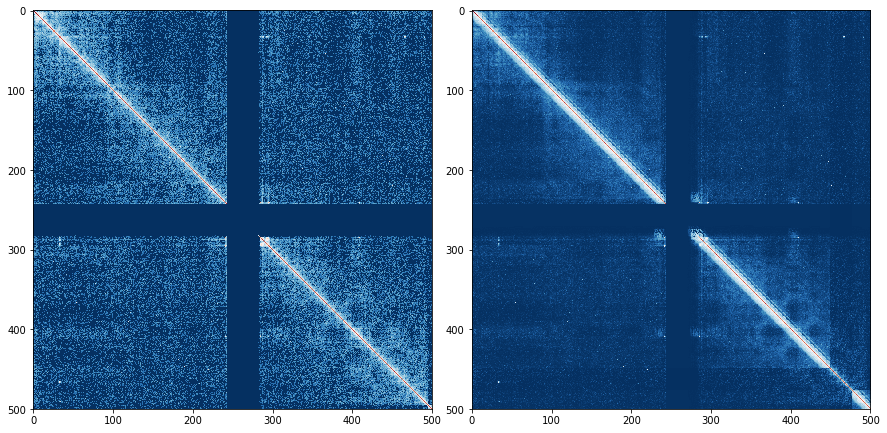
\includegraphics[width= 3.9in]{rl.png}}\\
        \subfloat[]{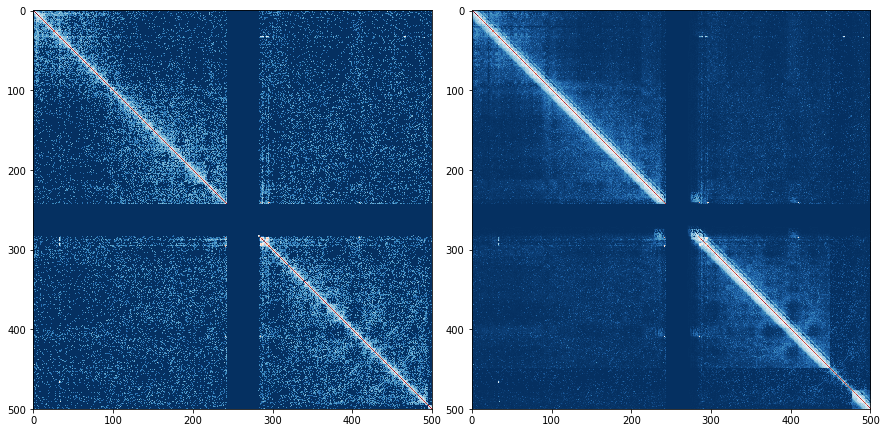
\includegraphics[width= 4in]{call4.png}}\\
        \caption{Results of running the model on
        cancer cells. For the
        sake of demonstration, we only show the
        firt 500 loci. The left contact matrices 
        are the 
        original low-resolution data and the rightmost
        pictures are the result of model predictions.}
        \label{fig:predict}
\end{figure}

\textbf{Platforms:}
The original model was developed in \texttt{theano} 
framework.
The package \texttt{lasagne} was used 
for model development. Although we made some experiments
with tensorflow, conducted our final traning via the
orginal model.
Our results can be found in a git repository (refer to
resources section).

We trained the model using low-resolution 
 GM06990 and high-resolution
 GM12878 data, both of which are sequence from
 the same cell. We then used the other three
 data that we have (corresponding to three
 cancerous cells) as input to the model to 
 improve contrast.
The data that we uses is described in table
\ref{tab:data}

The model was ran for 30 epochs. 
The results of training can be found in figure
\ref{fig:train}. As can be seen the results
are smoother and demonstrate higher contrast
than the original model.
Figure \ref{fig:predict} show prediction results
from the model for the three cancer cells. The
results also demonstrat higher contrast compared
to original contact matrices.



\section{Strengths and Weaknesses and Future Work}
This method can be considered as a noise reduction method
for Hi-C contact matrices. 
Just as all currently available
normalization and noise reduction approaches this method
also relies on assumptions. 
For example Balance Network Deconvolution,
proposed by \cite{feizi2013network}
assumes that the observed graph $G_{obs}$ is a summation of its
direct graph $G_{dir}$ and some indirect terms 
$G_{obs} = G_{dir} + G_{dir}^2 + G_{dir} + ...$ .
The major assumption of this
approach is that CNNs can predict values in high-resolution
matrix from the surrounding neighborhood in low-resolution
matrix. The difference of this assumption from other 
approaches is that it is easier to put the assumption to
statistical tests. Authors of \cite{zhang2018enhancing}
came to the conclusion that the assumption holds true for
a down-sampled version of high-resolution data. Whether
this is the case for an independent low-resolution data
remains to be investigated in future works.
\section{Resources}
\textbf{Source code for the project:}\\
\url{https://github.com/rasoolianbehnam/watson/tree/master/HiCPlus}\\
\textbf{Link to the low-resolution Hi-C datasets:}\\
\url{http://sysbio.rnet.missouri.edu/T0510/tmp_download/link_to_download_genome_data/contact_file/}\\
\textbf{Link to high-resolution Hi-C dataset:}\\
\url{https://www.ncbi.nlm.nih.gov/geo/query/acc.cgi?acc=GSE63525}

% MARK: bibliography
\bibliographystyle{my-unsrtnat}
\bibliography{references}


% MARK: acronyms
% a collection of Acronyms
\begin{acronym}
\acro{CNN}{Convolutional Neural Network}
\acro{GAN}{Generative Adversarial Network}
\end{acronym}

\end{document}
